\usepackage{fontspec}
\usepackage{mathtools}
\usepackage{unicode-math}
\usepackage{tikz}
\usetikzlibrary{trees}
\usepackage{mathpartir}
\usepackage{parskip}
\usepackage{minted}
\usepackage{csquotes}
\usepackage{tcolorbox}
\usepackage{biblatex} % TODO style w/o quotation marks
\usepackage{siunitx}
\usepackage{booktabs}
\usepackage{amsmath,amssymb}
\usepackage{color,soul}
\usepackage{xcolor}

\def\mul#1#2{\color{#1}\underline{{\color{black}#2}}\color{black}}

\newtheorem{lem}{Lemma}

\setmainfont{XITS}
\setmathfont{XITS Math}
\setsansfont[Scale=MatchLowercase]{DejaVu Sans}
\setmonofont[Scale=MatchLowercase]{DejaVu Sans Mono}

\addbibresource{lit.bib}

% Emoji images are from
% https://github.com/joypixels/emoji-assets/blob/master/png/128
\newlength{\emojiheight}
\settoheight{\emojiheight}{H}
\newcommand{\good}{\includegraphics[height=\emojiheight]{images/1f973}}
\newcommand{\bad}{\includegraphics[height=\emojiheight]{images/1fae4}}

\setbeamertemplate{navigation symbols}{}
\setbeamertemplate{itemize item}{\Large\textbullet}
\setbeamertemplate{itemize subitem}{\Large\textbullet}
\setbeamertemplate{itemize subsubitem}{\Large\textbullet}

\tcbset{frame empty}

\setminted[lean4]{extrakeywords={aesop cases add aesop? intro simp simp_all only split apply on_goal next rename_i safe unsafe norm constructors forward destruct norm_num done add_aesop_rules rfl subst ext}}
\newmintinline[lean]{lean4}{bgcolor={},ignorelexererrors=true}
\newminted[leancode]{lean4}{bgcolor={},ignorelexererrors=true,fontsize=\footnotesize,autogobble}
\BeforeBeginEnvironment{leancode}{\begin{tcolorbox}}
\AfterEndEnvironment{leancode}{\end{tcolorbox}}
\usemintedstyle{xcode}

\setlength{\parskip}{1em}
\setlength{\tabcolsep}{0.5em}

% Source: https://tex.stackexchange.com/questions/55806/mindmap-tikzpicture-in-beamer-reveal-step-by-step/55849#55849
%
% Keys to support piece-wise uncovering of elements in TikZ pictures:
% \node[visible on=<2->](foo){Foo}
% \node[visible on=<{2,4}>](bar){Bar}   % put braces around comma expressions
%
% Internally works by setting opacity=0 when invisible, which has the
% advantage (compared to \node<2->(foo){Foo} that the node is always there, hence
% always consumes space plus that coordinate (foo) is always available.
%
% The actual command that implements the invisibility can be overridden
% by altering the style invisible. For instance \tikzsset{invisible/.style={opacity=0.2}}
% would dim the "invisible" parts. Alternatively, the color might be set to white, if the
% output driver does not support transparencies (e.g., PS)
\tikzset{
  invisible/.style={opacity=0},
  visible on/.style={alt={#1{}{invisible}}},
  alt/.code args={<#1>#2#3}{%
    \alt<#1>{\pgfkeysalso{#2}}{\pgfkeysalso{#3}} % \pgfkeysalso doesn't change the path
  },
}

% Source: https://tex.stackexchange.com/questions/102069/make-a-heading-in-beamer
\newcommand\frameheading[1]{%
  \par\bigskip
  {\Large\usebeamercolor[fg]{palette primary}#1}\par\smallskip}

% Colourblind-friendly palette from https://www.nceas.ucsb.edu/sites/default/files/2022-06/Colorblind%20Safe%20Color%20Schemes.pdf
\definecolor{csgreen}{RGB}{000,158,115}
\definecolor{csorange}{RGB}{213,094,000}
\definecolor{csblue}{RGB}{000,114,178}
\definecolor{cspurple}{RGB}{204,121,167}
\newcommand{\orange}[1]{\textcolor{csorange}{#1}}
\newcommand{\blue}[1]{\textcolor{csblue}{#1}}
\newcommand{\grey}[1]{\textcolor{lightgrey}{#1}}
\newcommand{\green}[1]{\textcolor{csgreen}{#1}}
\newcommand{\purple}[1]{\textcolor{cspurple}{#1}}

\setbeamercolor{structure}{fg=csblue}

\renewcommand{\iff}{\leftrightarrow}
\newcommand{\com}{,\,}
\renewcommand{\emph}[1]{\blue{#1}}
\newcommand{\mv}[1]{\ensuremath{\mathit{?#1}}}
\newcommand{\rulename}[1]{\textrm{#1}}
\newcommand{\rulelabel}[1]{\quad \text{\rulename{#1}}}
\newcommand{\Expr}{\ensuremath{\mathbb{E}}}
\newcommand{\Hyps}{\ensuremath{\mathbb{H}}}
\newcommand{\Matches}{\ensuremath{\mathbb{M}}}
\newcommand{\Slots}{\ensuremath{\mathbb{S}}}
\newcommand{\Vars}{\ensuremath{\mathbb{V}}}
\newcommand{\Pow}[1]{\ensuremath{\mathcal{P}(#1)}}
\newcommand{\dom}[1]{\ensuremath{\mathrm{dom}(#1)}}
\newcommand{\cod}[1]{\ensuremath{\mathrm{cod}(#1)}}
\newenvironment{rapppic}{\begin{tikzpicture}[outer sep=auto, level distance=3em]}{\end{tikzpicture}}
\newenvironment{rapp}{%
  \begin{tcolorbox}
  \begin{center}
  \begin{rapppic}
}{
  \end{rapppic}
  \end{center}
  \end{tcolorbox}%
}


% Theme choice:
\usetheme{default}

% Title page details: 
\title{For­mal­iza­tion of Drin­feld Mod­ules} 
\author{Xavier Généreux}
\date[\today]{\today \\ \vspace{1cm} Joint work with María Inés de Frutos-Fernández}
\logo{
\includegraphics[width=3cm]{images/Logo_LMU.png}}
\institute 
{
	Lean­ing In! 2025
}


\begin{document}

% Title page frame
\begin{frame}
    \titlepage 
\end{frame}

% Remove logo from the next slides
\logo{}


% Outline frame
\begin{frame}{Plan for today}
	\begin{itemize}
		\item Some motivation
		\item The definition of Drinfeld Modules
		\item The formalization
	\end{itemize}
\end{frame}

\begin{frame}{Motivation}
	\framesubtitle{Shutting down reactors?}
	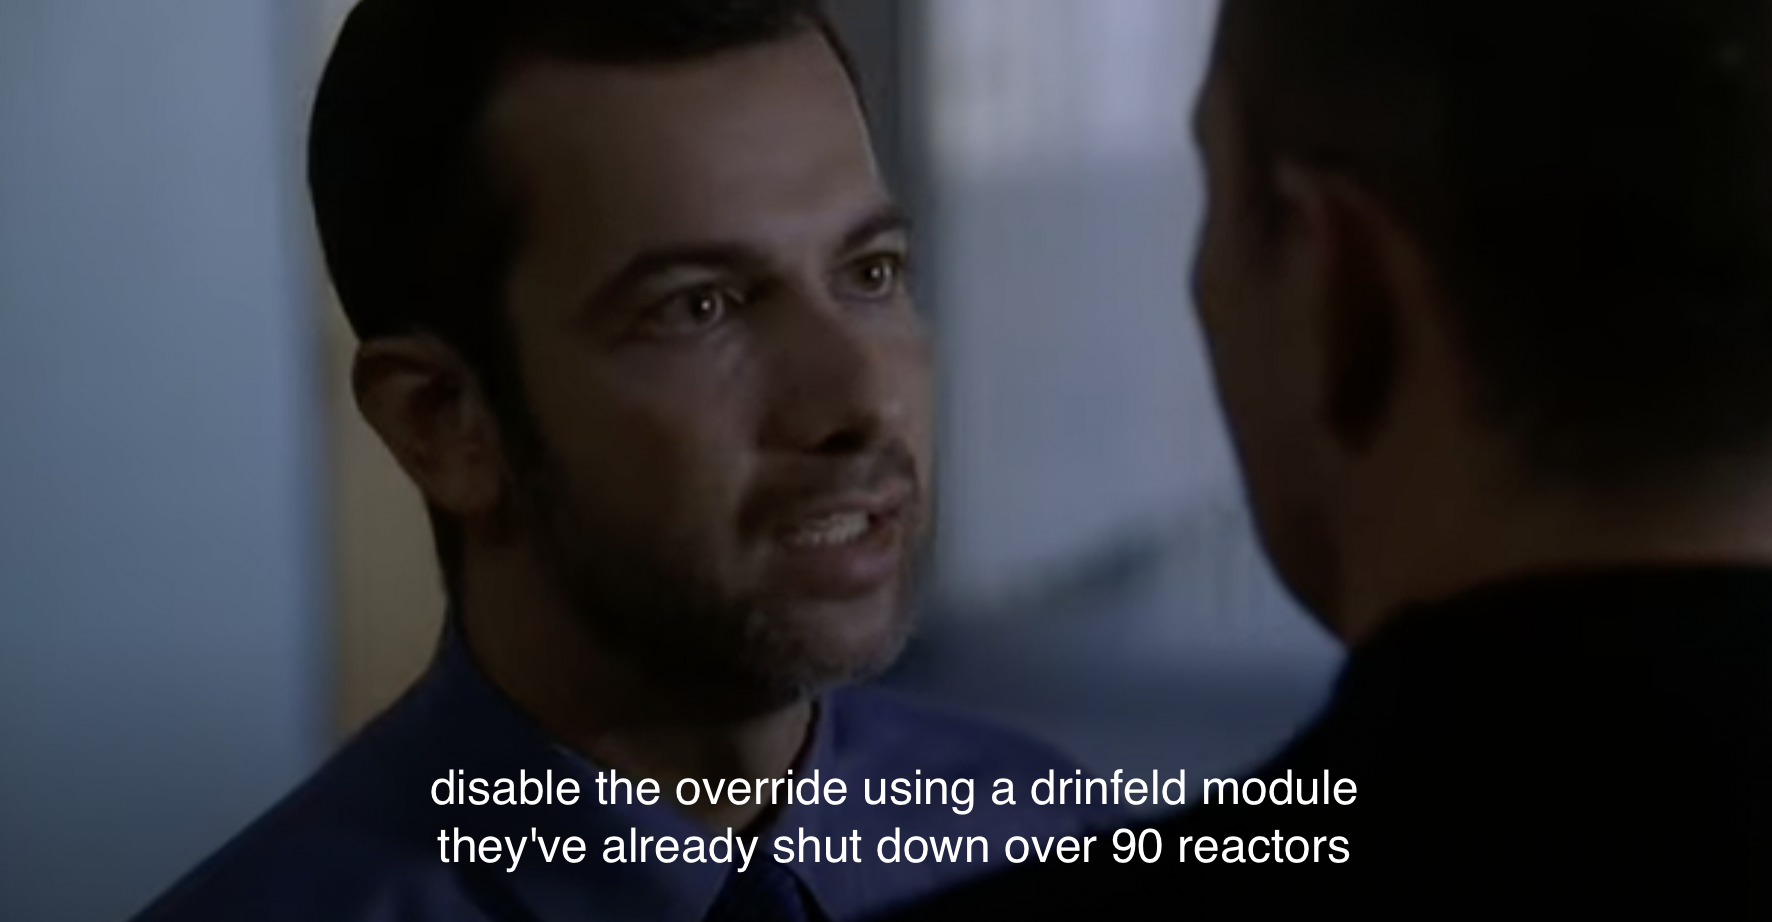
\includegraphics[width=10.5cm]{images/drinfeld_module_24.png}
	From Fox's 2005 tv show "24", Season 4 Episode 11 .
\end{frame}

% \begin{frame}{Motivation}
% 	\framesubtitle{Can Wikipedia help us?}
% 	From Wikipedia: 

%   \
% 	\begin{quote}
%         ``Drinfeld module is roughly a special kind of module \pause over a ring of functions \pause on a curve \pause over a finite field.''
%     \end{quote}
% \end{frame}

\begin{frame}{Motivation}
	\framesubtitle{The Function Field Analogy}
	Let $q = p^n$ for some prime $p$.
	We have the following correspondence :

	\begin{align*}
		&\mathbb{Z} & &\mapsto & &\mathbb{F}_q[T]
		& &\only<1>{\text{ (The polynomials over } \mathbb{F}_q.)} \\
		&\only<2->{\mathbb{Q} & &\mapsto & &\mathbb{F}_q(T)}
		& &\only<2>{\text{(The rational functions over } \mathbb{F}_q.)} \\
    \only<3->{K &/ \mathbb{Q} & &\mapsto & &K / \mathbb{F}_q(T)}
		& &\only<3>{\text{(Finite algebraic extensions.)}} \\
		&\only<4->{\mathbb{\overline{Q}} & &\mapsto & &\overline{\mathbb{F}_q(T)}}
		& &\only<4>{\text{(The algebraic closure of } \mathbb{F}_q(T).)}\\
		\only<5->{|&\cdot| & &\mapsto & &|\cdot|_\infty}
		& &\only<5>{(\text{where } |\cdot|_\infty = q^{\text{deg}(\cdot)}.)}\\
            &\only<6->{\mathbb{R} & &\mapsto & &\mathbb{F}_q((1/T))}
		& &\only<6>{\text{(The completion of } \mathbb{F}_q(T).)}\\
		&\only<7->{\mathbb{C} & &\mapsto & &\widehat{\overline{\mathbb{F}_q((1/T))}}}
		& &\only<7>{\text{(Take closure + completion.)}}
	\end{align*}

  \only<8>{
  Fields $K/\mathbb{F}_q(T)$ are \textit{Function Fields}.}
\end{frame}



\begin{frame}{Motivation}
	\framesubtitle{The Function Field Analogy}
	
	This is an analogy in the sense that the objects on both sides share a lot of properties.
  
  However, proofs are somewhat "easier" in function fields.
	
	\pause
	\

	Notably, the following is proven over function fields:
	\begin{enumerate}
		\item The extended Riemann hypothesis.
		\pause 
		\item The Langlands program for $\text{GL}_n$.
	\end{enumerate}
\end{frame}



\begin{frame}{Motivation}
	\framesubtitle{The exponential}
	
	Carlitz in 1935 extended the function field analogy by attaching an \textit{exponential function} $e_C(z)$.

	\

	This function shares many interesting properties with $e^z$.
	However, 
	$$e^{nz} = (e^z)^n$$
	the Carlitz exponential satisfies
	$$e_C(az) = C_a(e_C(z)), \text{ for } a \in F_q[T].$$

	\pause

	Here, $C_a(u)$ is an additive polynomial which means that
	$$C_a(u + v) = C_a(u) + C_a(v)$$.
\end{frame}

\begin{frame}{Motivation}
	\framesubtitle{The Carlitz Module}
	
	The mapping $a \mapsto C_a(u)$ is the simplest example of a Drinfeld Module. (Which we call the Carlitz Module.)

	\pause
	\

	In his paper, Drinfeld extended this idea to general exponential functions of \textbf{arbitrary rank} $d$ (where $e_C(z)$ has rank 1) associated to an \textbf{arbitrary function field} with an \textbf{arbitrary choice of place} $\infty$.

	It is using generalizations of these constructions that the Langlands program for $\text{GL}_n$ over function fields was realized. (Due to Drinfeld for $\text{GL}_2$ and Lafforgue for $\text{GL}_n$.)

\end{frame}

\begin{frame}{The Definition}
	\framesubtitle{Skew Polynomials}
	
	Let $R$ be some commutative $\mathbb{F}_q$-algebra. The set $R\{\tau\}$ given by polynomials $\sum_{i\geq 0}^n a_i \tau^i, a_i \in R$ is a ring with the usual addition and where the multiplication is given by
	
	$$\tau  a = a^{q}\tau.$$

	This multiplication extends to all polynomial via distributivity laws.

\end{frame}

\begin{frame}[fragile]{The Definition}
	\framesubtitle{Skew Polynomials}
	
	We have defined skew polynomial
        \begin{minted}{lean}
def SkewPolynomial (R : Type*) [AddCommMonoid R] := ...
        \end{minted}
	which respects the expected identity
	\begin{minted}{lean}
lemma X_pow_mul_monomial (k n : Nat) (r : R) :
   X^k * monomial n r = monomial (n+k) (f^[k] r) := ...
	\end{minted}
    
        \ 
        
        Note that in our case, $f := a \mapsto a^q$.
\end{frame}

\begin{frame}[fragile]{The Definition}
	\framesubtitle{$\mathbb{F}_q$-linear polynomials}
        Let $K$ be a field containing $\mathbb{F}_q$. The following,
        $$K\langle x \rangle = \left\{\sum_{i = 0}^n a^i x^{q^i} | a_i \in K \right\},$$
        is called the ring of $\mathbb{F}_q$-linear polynomials.
        It is a ring with the usual addition and where the multiplication is given by \textit{composition}.
        
        We have the following isomorphism
        $$K\{\tau\} \cong K\langle x \rangle$$
        $$\sum_{i = 0}^n a_i \tau^{i} \mapsto \sum_{i = 0}^n a_i x^{q^i}$$
        Given $f \in K\{\tau\}$, we write $f(x)$ for its image through the isomorphism.
\end{frame}

% \begin{frame}[fragile]{The Definition}
% 	\framesubtitle{Drinfeld Modules}
%         Instead of $\mathbb{F}_q[T]$, we consider $A$ the ring of regular functions outside of $\infty$.
        
%         Let $\mathcal{F}$ be a field equipped with a fixed morphism $\iota : A \to \mathcal{F}$.
	
% 	\begin{definition}
%             A \textit{Drinfeld Module} is a $\mathbb{F}_q$-algebra homomorphism 
%             $$\phi : A \to \mathcal{F}\{\tau\}$$
%             such that
%             \begin{enumerate}
%                 \item $D \circ \phi = \iota$;
%                 \item for some $a \in A, \phi(a) \neq \iota(a)\tau^0$.
%             \end{enumerate}
%         \end{definition}
% \end{frame}

\begin{frame}[fragile]{The Definition}
	\framesubtitle{Drinfeld Modules}
  Let $\mathcal{F}$ be a field equipped with a fixed morphism $\iota : \mathbb{F}_q[T] \to \mathcal{F}$.
	
	\begin{definition}
            A \textit{Drinfeld Module} is a $\mathbb{F}_q$-algebra homomorphism 
            $$\phi : \mathbb{F}_q[T] \to \mathcal{F}\{\tau\}$$
            for which there exists $a_1,\dots,a_r$ not all zero such that
            $$\phi_T = \iota(T) + a_1\tau + \dots + a_r\tau^r.$$
        \end{definition}
        \pause
        The $\mathbb{F}_q[T]$-module structure on $\mathcal{F}$ is given by $a * f = \phi_a(f)$.  
\end{frame}

\begin{frame}[fragile]{The Definition}
	\framesubtitle{Drinfeld Modules in lean}

We formalize a slightly more general version where \mintinline{lean}{IsCoeffRing} generalizes the ring $\mathbb{F}_q[T]$.

        \begin{minted}{lean}
structure DrinfeldModule {A : Type} [CommRing A]
    [Algebra A F] [IsCoeffRing F v A] (ι : A →+* R)
    extends A →+* (SkewPolynomial R) where
  derivative : (coeff · 0).comp toFun = ι
  nontrivial : toFun ≠ C.comp ι
        \end{minted}
\end{frame}

\begin{frame}{Formalization}
	\framesubtitle{Ostrowski's Theorem for $\mathbb{F}_q(T)$}

        \begin{theorem}
            Any nontrivial absolute value on $\mathbb{F}_q(T)$ is equivalent to $| \cdot |_\infty$ or to $| \cdot |_p$ for some monic irreducible $p$ in $\mathbb{F}_q[T]$.
        \end{theorem}
        \ 
        
        Accessible because :
        \begin{enumerate}
            \item Good proof script already exists. [2]
            \item \textbf{All} relevant definitions were already in Mathlib.
            \item \textbf{Many} of the required lemmas were already in Mathlib.
            \item Good API.
        \end{enumerate}
\end{frame}

\begin{frame}[fragile]{Formalization}
	\framesubtitle{Ostrowski's Theorem for $\mathbb{F}_q(T)$}

        What I mean by good API:
        \begin{itemize}
            \item Induction principle takes proofs from $\mathbb{F}_q(T)$ to $\mathbb{F}_q[T]$.
            \item Mathlib can do "basic" mathematical reasoning :

            \ 

            \begin{quote}
                If there exists a polynomial $f(x)$ s. t. $|f(x)| < 1$, we can find a polynomial $f'(x)$ of least degree s. t. $|f'(x)| <1 $.
            \end{quote}
            Given in Mathlib by \mintinline{lean}{WellFounded.min}.
            
        \end{itemize}
\end{frame}

\begin{frame}[fragile]{Formalization}
	\framesubtitle{\mintinline{lean}{SkewPolynomial} and \mintinline{lean}{SkewMonoidAlgebra}}

        Goal : Translate most of Mathlib's results for polynomials and monoid algebras.

        Challenges :
        \begin{itemize}
            \item This is a big fragment to translate ($\sim$ 2400 lines)
            \item We would like to mirror the implementation of polynomials and monoid algebras.
        \end{itemize}
\end{frame}

\begin{frame}[fragile]{Formalization}
	\framesubtitle{\mintinline{lean}{SkewPolynomial} and \mintinline{lean}{SkewMonoidAlgebra}}

        In Mathlib, polynomial are defined as
\begin{minted}{lean}
structure Polynomial (R : Type*) [Semiring R] where
  ofFinsupp :: toFinsupp : AddMonoidAlgebra R ℕ
\end{minted}
where 
\begin{minted}{lean}
def AddMonoidAlgebra :=
  G →₀ k
\end{minted}
    
\end{frame}

\begin{frame}[fragile]{Formalization}
	\framesubtitle{\mintinline{lean}{SkewPolynomial} and \mintinline{lean}{SkewMonoidAlgebra}}

However, there is a planned refactor to restore \mintinline{lean}{Polynomial} as a definition and put \mintinline{lean}{AddMonoidAlgebra} in a structure.

This is what we have done in the skewed case:
\begin{minted}{lean}
def SkewPolynomial (R : Type*) [AddCommMonoid R] :=
  SkewMonoidAlgebra R (Multiplicative ℕ)
\end{minted}
where 
\begin{minted}{lean}
structure SkewMonoidAlgebra (k G : Type*) [Zero k] where
  /-- Map **from** `G →₀ k`. -/
  ofFinsupp ::
  /-- Map **to** `G →₀ k`. -/
  toFinsupp : G →₀ k
\end{minted}
\end{frame}

\begin{frame}[fragile]{Formalization}
	\framesubtitle{Using the universal property}

Instead of stating theorem in terms of \mintinline{lean}{RatFunc F}, we can state theorems in terms of \mintinline{lean}{K} with the instance \mintinline{lean}{[IsFractionRing F[X] K]}.

\pause

\

This allows one to use seemlessly result for \mintinline{lean}{RatFunc F} but also for \mintinline{lean}{FractionRing F[X]}.

\end{frame}

\begin{frame}[fragile]{Formalization}
	\framesubtitle{Using the universal property}

In our project, we could have defined Drinfeld modules as 

        \begin{minted}{lean}
structure DrinfeldModule (ι : (CoeffRing F v) →+* R)
    extends (CoeffRing F v) →+* (SkewPolynomial R) where
  derivative : (coeff · 0).comp toFun = ι
  nontrivial : toFun ≠  C.comp ι
        \end{minted}

\end{frame}

\begin{frame}[fragile]{Formalization}
	\framesubtitle{Using the universal property}

But instead we choose

        \begin{minted}{lean}
structure DrinfeldModule {A : Type} [CommRing A]
    [Algebra A F] [IsCoeffRing F v A] (ι : A →+* R)
    extends A →+* (SkewPolynomial R) where
  derivative : (coeff · 0).comp toFun = ι
  nontrivial : toFun ≠ C.comp ι
        \end{minted}

\pause

In particular, this means that we can instantiate the definition with
$\mathbb{F}_q[T]$ which is an instance of \mintinline{lean}{[IsCoeffRing _ _ _]} but not equal to \mintinline{lean}{CoeffRing}.

\end{frame}

\begin{frame}[fragile]{Formalization}
	\framesubtitle{Other challenges}

\begin{itemize}
    \item Towers of fields.
    \item Arguments from the theory that we can't follow.
    \item A ``straighforward'' way to talk about $K[X,Y]$.
\end{itemize}

\end{frame}

\begin{frame}[fragile]{Thank you!}

 \footnotesize
    [1] Goss, David. “Basic Structures of Function Field Arithmetic.” (1997). \\
    
    [2] Conrad, Keith. ``Ostrowski's theorem for F(T).'' (accessed online).\\
    
    [3] Rosen, Michael I.. “Number Theory in Function Fields.” (2002).\\
  
    [4] Papikian, Mihran. “Drinfeld Modules.” (2023).

\end{frame}

\end{document}